\documentclass{bredelebeamer}
\usepackage{subfig}

%%%%%%%%%%%%%%%%%%%%%%%%%%%%%%%%%%%%%%%%%%%%%%%%
\title[Ingénierie dirigée par les Modèles]{IDM - Soutenance 3}
% Titre du diaporama

\subtitle{Groupe 1 - Les roboticiens}
% Sous-titre optionnel

\author{N. Salleron Y. Ghigoff K. Vu-Saintonge A. Archambault}
% La commande \inst{...} Permet d'afficher l' affiliation de l'intervenant.
% Si il y a plusieurs intervenants: Marcel Dupont\inst{1}, Roger Durand\inst{2}
% Il suffit alors d'ajouter un autre institut sur le modéle ci-dessous.

\date{29 Janvier 2018}
% Optionnel. La date, généralement celle du jour de la conférence

\subject{IDM}
% C'est utilisé dans les métadonnes du PDF

\logo{

\includegraphics[scale=0.03]{images/logo.jpg}
}

%%%%%%%%%%%%%%%%%%%%%%%%%%%%%%%%%%%%%%%%%%%%%%%%%%%%%%%%%%%%%%%%%%%%%
\begin{document}

\begin{frame}
  \titlepage
\end{frame}

\begin{frame}{Sommaire}
  \tableofcontents
  % possibilité d'ajouter l'option [pausesections]
\end{frame}

\section{Introduction}
\subsection{Introduction}


\begin{frame}{Introduction}
%Texte normal \alert{Texte Alert}  \exemple{Texte exemple} \emph{Texte emphase}
\begin{columns}
\begin{column}{0.5\textwidth}
\begin{alertblock}{Contexte}
\begin{itemize}
\item Domaine de la danse.
\item Préparation d'une chorégraphie et exécution sur le terrain.
\item Création d'un langage de programmation spécifique.
\end{itemize}
\end{alertblock}
\begin{block}{Objectif}
\begin{itemize}
\item Produire un langage de programmation \alert{simple} et \alert{compréhensible} pour l'utilisateur.
\item Rendre l'utilisateur autonome.
\item Adaptable à  plusieurs drones.
\item Faire danser le drone.
\end{itemize}
\end{block}
\end{column}
\begin{column}{0.5\textwidth}
\begin{figure}
\centering
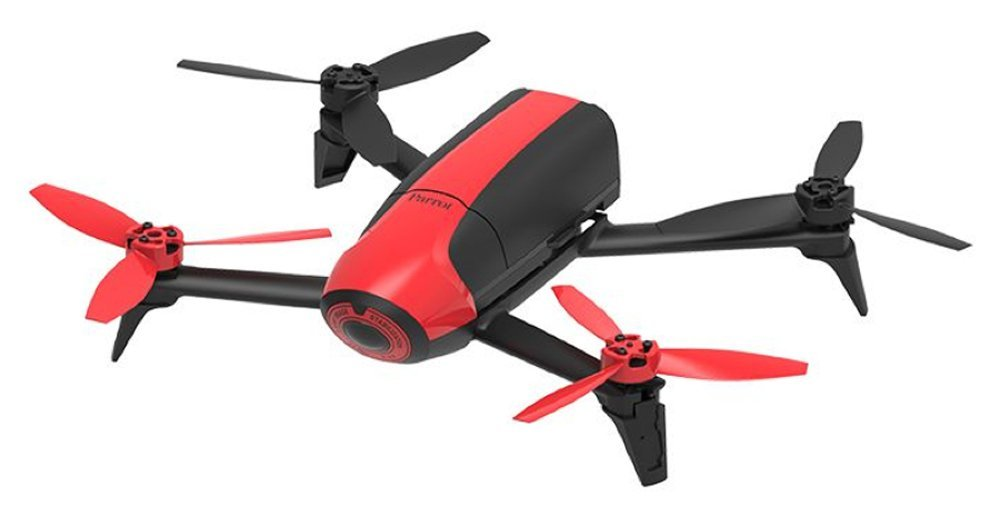
\includegraphics[scale=0.15]{images/img1.jpg}
\caption{Exemple de drone}
\end{figure}
\end{column}
\end{columns}
\end{frame}

\subsection{Rappel des tranches}

\begin{frame}{Tranches}
\begin{block}{But des tranches}
\begin{itemize}
\item 4 Tranches distinctes.
\item Associées à des dates de livraison.
\item Chacune ayant plusieurs objectifs à remplir.
\end{itemize}
\end{block}

\pause

\begin{exampleblock}{Vérification des tranches}
\begin{itemize}
\item Tests unitaires réalisés par l'équipe.
\item Mise en en place de test de validation.
\item Détaillés dans le cahier des charges.
\end{itemize}
\end{exampleblock}
\end{frame}

\begin{frame}{Tranches 0 et 1}
\begin{alertblock}{Objectifs de la Tranche 0}
\begin{itemize}
\item Analyse de la demande  par l'équipe.
\item Discussion avec le client.
\item Rédaction et rendu du cahier des charges.
\end{itemize}
\end{alertblock}

\pause

\begin{alertblock}{Objectifs de la Tranche 1}
\begin{itemize}
\item Création d'une grammaire pour DSL.
\item Création de l'éditeur associé.
\item Vérification des erreurs (syntaxiques, cycles...).
\end{itemize}
\end{alertblock}

\pause

\begin{block}{Retours du client}
\begin{itemize}
\item Syntaxe élégante (notamment sur les mouvements parallèles).
\item Changement sur l'intégration des bibliothèques de fonction et leur utilisation.
\item Changement sur l'appel de fonction dans une fonction (détection de cycle).
\end{itemize}
\end{block}
\end{frame}

\begin{frame}{Tranche 2}
\begin{alertblock}{Objectifs}
\begin{itemize}
\item Génération de code JAVA.
\item Création d'une interface de Runtime pour gérer plusieurs API de drone.
\item Affichage textuel des commandes qui seront envoyées au drone.
\end{itemize}
\end{alertblock}

\pause

\begin{block}{Retours du client}
\begin{itemize}
\item Tranche satisfaisante.
\item Création d'un bouton pour la génération du code (éviter de générer le code trop souvent).
\end{itemize}
\end{block}
\end{frame}

\begin{frame}{Tranche 3}
\begin{alertblock}{Objectifs}
\begin{itemize}
\item Liaison de notre interface avec la runtime du Parrot.
\item Déployer la solution sur un ordinateur d'exécution (notre ordinateur ou celui du client).
\item Test de la solution (recette).
\end{itemize}
\end{alertblock}
\end{frame}

\section{Editeur de langage}
\subsection{L'éditeur}

\begin{frame}{Editeur de langage}
\begin{columns}
\begin{column}{0.5\textwidth}
\begin{block}{Description de l'éditeur}
Notre éditeur possède les fonctionnalités suivantes :
\begin{itemize}
\item Auto-complétion du langage. 
\item Détection des fautes syntaxiques.
\item Détection des erreurs de cohérence dans les scénarios.
\end{itemize}
\end{block}\pause


\begin{block}{Ecriture de la chorégraphie}
\begin{itemize}
\item L'utilisateur écrit sa chorégraphie par une suite d'actions séparées par un retour à  la ligne.
\item Une chorégraphie commence par un décollage et un atterrissage.
\item Usage possible de fonctions et d'instructions simples.
\end{itemize}
\end{block}\pause
\end{column}
\begin{column}{0.5\textwidth}
\begin{alertblock}{Conditions de fonctionnement}
\begin{itemize}
\item Le drone utilisé est un drone à  hélices. 
\item Le drone est allumé, connecté via Wi-Fi à l'ordinateur.
\item Java version 1.8. 
\item Système d'exploitation MacOS et Linux.
\end{itemize}
\end{alertblock}
\vspace{80px}
\end{column}
\end{columns}
\end{frame}



\section{Fonctionnement du drone}
\subsection{Mouvements considérés}

\begin{frame}{Drone}

\begin{columns}

\begin{column}{0.65\textwidth}

\begin{block}{Mouvements sur les axes}
Le drone évoluant dans un environnement 3D, ce dernier peut effectuer différentes actions: \\
\begin{itemize}
\item Altitude : évolution sur l'axe Z. \\Correspond aux instructions "\alert{monter}" et "\alert{descendre}"
\item Roll : évolution sur l'axe X. \\Correspond aux instructions "\alert{gauche}" et "\alert{droite}"
\item Pitch: évolution sur l'axe Y. \\Correspond aux instructions "\alert{avancer}" et "\alert{reculer}"
\end{itemize}
\end{block}\pause

\begin{exampleblock}{Eléments particuliers}
\begin{itemize}
\item Décollage et Attérrissage : correspond aux instructions "\alert{decoller}" et "\alert{atterrir}"
\item Pause : correspond à  l'instruction "\alert{pause}"
\item Rotation : correspond aux instructions "\alert{rotationGauche}" et "\alert{rotationDroite}"
\end{itemize}
\end{exampleblock}\pause

\end{column}
\begin{column}{0.35\textwidth}
\begin{alertblock}{Cas de la caméra}
\begin{itemize}
\item Caméra : Il n'est pas standard qu'un drone posséde une caméra.
\end{itemize}
\end{alertblock}
\begin{figure}
\centering
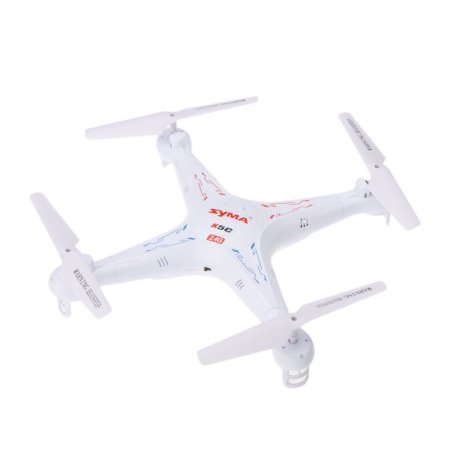
\includegraphics[scale=0.20]{images/img3.jpeg}
\caption{Exemple de drone sans caméra}
\end{figure}
\vspace{15px}
\end{column}
\end{columns}
\end{frame}

\section{Commandes du DSL}
	\subsection{Prologue}

\begin{frame}[fragile]{Prologue}
\begin{block}{Définir 5 constantes de vol}
\begin{itemize}
\item \alert{define} \emph{vitesse\_hauteur\_max}: vitesse maximale d'élévation du drone pour la chorégraphie.
\item \alert{define} \emph{vitesse\_deplacement\_max}: vitesse maximale de déplacement sur le plan horizontal du drone pour la chorégraphie. 
\item \alert{define} \emph{vitesse\_rotation\_max}: vitesse maximale de rotation du drone pour la chorégraphie.
\item \alert{define} \emph{hauteur\_max}: Cette constante permet de limiter l'altitude maximale du drone en vol.
\item \alert{define} \emph{eloignement\_max}: Cette constante permet de contr\^oler la distance horizontale du drone en vol par rapport au point de décollage.
\end{itemize}
\end{block}


Exemple de define : 
\begin{center}
\color{Framarouge}
	define vitesse\_hauteur\_max \color{Framagris}50\%
\end{center}
\end{frame} 

	\subsection{Instructions basiques} 
\begin{frame}{Instructions basiques} 
Le but est de rendre accessible le pilotage de drone aux chorégraphes. 
\begin{block}{Les 11 instructions basiques}
\begin{itemize}
\item \alert{decoller} et \alert{atterrir}
\item \alert{pause(durée : Seconde)}
\item \alert{monter(durée : Seconde, vitesse\_verticale : Pourcentage)}
\item \alert{decendre(durée : Seconde, vitesse\_verticale : Pourcentage)}
\item \alert{avancer(durée : Seconde, vitesse\_deplacement : Pourcentage)}
\item \alert{reculer(durée : Seconde, vitesse\_deplacement : Pourcentage)}
\item \alert{gauche(durée : Seconde, vitesse\_deplacement : Pourcentage)}
\item \alert{droite(durée : Seconde, vitesse\_deplacement : Pourcentage)}
\item \alert{rotationGauche(durée : Seconde, vitesse\_rotation : Pourcentage)}
\item \alert{rotationDroite(durée : Seconde, vitesse\_rotation : Pourcentage)}
\end{itemize}
\end{block}
\begin{itemize}
\item 1er paramètre est la durée du mouvement, en Seconde.
\item 2eme paramètre est la vitesse du mouvement, en pourcentage. \\Il représente la vitesse du drone par rapport à  la vitesse définie dans \\la section "prologue".
\end{itemize}
\end{frame}

	\subsection{Instructions parallèles} 
\begin{frame}{Les Instructions parallèles} 
\begin{itemize}
\item Notre langage intègre un mécanisme d'exécution d'instructions parallèles.
\item Il est possible d'ordonner au drone de faire plusieurs instructions en même temps. 
\item Mécanisme implémenté par le symbole '\&'. \pause
\item Disponible que pour certaines instructions comme :  
	\begin{enumerate}
		\item monter
		\item descendre
		\item avancer
		\item reculer
		\item gauche
		\item droite
		\item rotationGauche
		\item rotationDroite
	\end{enumerate}	\pause
\item Maximum de 4 instructions parallélisables.
\end{itemize}
Exemple : \newline
\color{Framarouge}rotationDroite(\color{black}2\color{Framarouge},\color{Framagris}25\%\color{Framarouge}) \& 
	\color{Framarouge}avancer(\color{black}5\color{Framarouge},\color{Framagris}20\%\color{Framarouge})\\ \pause
	\color{black}-> Ok \newline
	\color{Framarouge}monter(\color{black}1\color{Framarouge},\color{Framagris}10\%\color{Framarouge}) \& 
	\color{Framarouge}descendre(\color{black}4\color{Framarouge},\color{Framagris}20\%\color{Framarouge})\\ \pause
	\color{black}-> Impossible les deux commandes s'opposent.\\
	\color{Framarouge}gauche(\color{black}3\color{Framarouge},\color{Framagris}25\%\color{Framarouge}) \& 
	\color{Framarouge}gauche(\color{black}4\color{Framarouge},\color{Framagris}20\%\color{Framarouge})\\ \pause
	\color{black}-> Impossible les deux commandes sont de même type.\\

\end{frame}
	
	\subsection{Fonctions} 
\begin{frame}{Les fonctions} 
\begin{itemize}
\item Le langage permet de définir des fonctions.
\item Les fonctions sont une suite d'instructions séquentielles.
\item Il n'est pas possible de paralléliser deux fonctions.
\item Une fonction ne peut pas s'appeler elle-même et les cycles ne sont pas autorisés.
\end{itemize}


\begin{tabbing}
Exemple : \=\\
	\>\color{Framarouge}func \=\color{black}maFonction\color{Framarouge}() \{\\ 
	\>\>\color{Framarouge}rotationDroite(\color{black}2\color{Framarouge},\color{Framagris}25\%\color{Framarouge}) \& 
	\color{Framarouge}avancer(\color{black}5\color{Framarouge},\color{Framagris}20\%\color{Framarouge})\\ 
	\>\>\color{Framarouge}droite(\color{black}3\color{Framarouge},\color{Framagris}80\%\color{Framarouge})\\ 
	\>\>\color{Framarouge}avancer(\color{black}4\color{Framarouge},\color{Framagris}10\%\color{Framarouge})\\ 
	\>\color{Framarouge}\}
\end{tabbing}
\begin{tabbing}
Exemple \=ne fonctionnant pas: \\
	\>\color{Framarouge}func \=\color{black}A\color{Framarouge}() \{\\ 
	\>\>\color{Framarouge}B() \color{black} //Erreur sur B() \\
	\>\color{Framarouge}\} \\
	\>\color{Framarouge}func \=\color{black}B\color{Framarouge}() \{\\ 
	\>\>\color{Framarouge}A()  \color{black} //Erreur sur A()\\
	\>\color{Framarouge}\}
\end{tabbing}

\end{frame}

\subsection{Le bloc "main" et les bibliothèques de fonctions} 
\begin{frame}{Le bloc "main" et les bibliothèques de fonctions} 

\begin{columns}

\begin{column}{0.5\textwidth}


Le point d'entrée "main \{ \}" :\\
\begin{itemize}
\item Défini par le mot clé "main"
\item Le contenu de ce bloc d'instructions sera exécuté.
\item Il est le seul à  pouvoir appeler des fonctions.
\end{itemize}\pause

\begin{tabbing}
Exemple :\=\\
	\>\color{Framarouge}main  \{\=\\ 
	\>\>\color{Framarouge}decoller()\\
	\>\>\color{Framarouge}gauche(\color{black}1\color{Framarouge},\color{Framagris}10\%\color{Framarouge})\\ 
	\>\>\color{Framarouge}avancer(\color{black}4\color{Framarouge},\color{Framagris}34\%\color{Framarouge})\\
	\>\>\color{Framarouge}maFonction()\\ 
	\>\>\color{Framarouge}atterrir()\\
	\>\color{Framarouge}\}\\
	
	\>\color{Framarouge}func \=\color{black}maFonction\color{Framarouge}() \{\\ 
	\>\>\color{Framarouge}rotationDroite(\color{black}2\color{Framarouge},\color{Framagris}25\%\color{Framarouge}) \& 
	\color{Framarouge}avancer(\color{black}5\color{Framarouge},\color{Framagris}20\%\color{Framarouge})\\ 
	\>\>\color{Framarouge}droite(\color{black}3\color{Framarouge},\color{Framagris}80\%\color{Framarouge})\\ 
	\>\>\color{Framarouge}avancer(\color{black}4\color{Framarouge},\color{Framagris}10\%\color{Framarouge})\\ 
	\>\color{Framarouge}\}\pause

\end{tabbing}	
\end{column}
\begin{column}{0.5\textwidth}
Les bibliothèques de fonctions:\\
\begin{itemize}
\item Possibilité d'utiliser des fonctions définies dans des fichiers .lib\_drone.
\item Doivent être dans le même répertoire que le fichier appelant les fonctions.
\end{itemize}\pause
\begin{tabbing}
Exemple :\=\\
            \>\color{Framarouge}import <\color{black}monFichier.lib\_drone\color{Framarouge}>\pause
\end{tabbing}		
\vspace{10px}
Utilisation du nom de fichier (ici : \color{Framarouge}monFichier\color{black}) pour référencer la fonction de la bibliothèque que nous souhaitons utiliser.
\begin{tabbing}
Exemple :\=\\
            \>\color{Framarouge}import <\color{black}monFichier.lib\_drone\color{Framarouge}>\\
	    	\>\color{Framarouge}main  \{\=\\ 
	\>\>\color{Framarouge}decoller()\\
	\>\>\color{black}monFichier.toto()\\ 
	\>\>\color{Framarouge}atterrir()\\
	\>\color{Framarouge}\}\\
\end{tabbing}


\end{column}
\end{columns}

\end{frame}



\section{Environnement}

	\subsection{Explications}
\begin{frame}{Environnement}
\begin{block}{Application}
\begin{itemize}
\item Disponible sur MacOS.
\item Disponible sur Linux.
\end{itemize}
\end{block}\pause
\begin{figure}
\centering
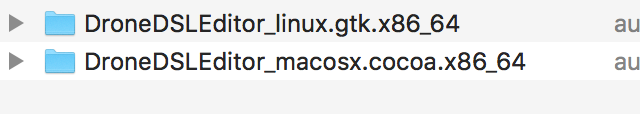
\includegraphics[scale=0.7]{images/Distrib.png}
\caption{Distributions}
\end{figure}
\end{frame}
    
\begin{frame}{Environnement}
\begin{block}{Lancement de l'environnement : exemple sous MacOS}
\begin{itemize}
\item Lancement de l'application via le script DroneDSLEditor.sh \pause
\begin{enumerate}
\item Vérification des dépendances (seulement la première fois)\pause
\item Compilation du SDK (seulement la première fois)\pause
\item Lancement de l'application\pause
\end{enumerate}
\end{itemize}
\end{block}
\begin{figure}
\centering
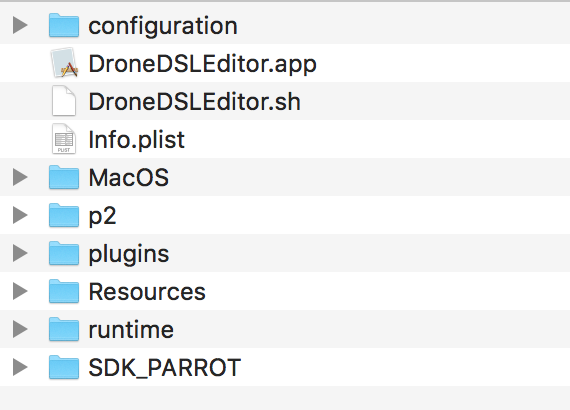
\includegraphics[scale=0.3]{images/Contenu.png}
\caption{Lancement de l'application}
\end{figure}
\end{frame}

\begin{frame}{Environnement}
\begin{block}{Création d'un projet}
\begin{itemize}
\item Via l'interface graphique (file -> new -> project).
\end{itemize}
\end{block}\pause
\begin{figure}
\centering
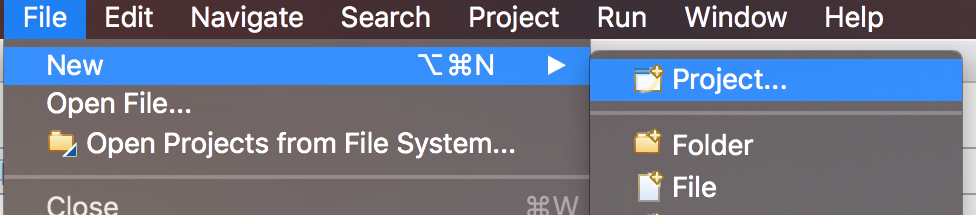
\includegraphics[scale=0.21]{images/04.png}
\caption{Création d'un nouveau projet}
\end{figure}
\end{frame}

\begin{frame}{Environnement}
\begin{block}{Création d'un projet}
\begin{itemize}
\item Créer un projet Xtext nommé DroneDSL Project.
\end{itemize}
\end{block}\pause
\begin{figure}
\centering
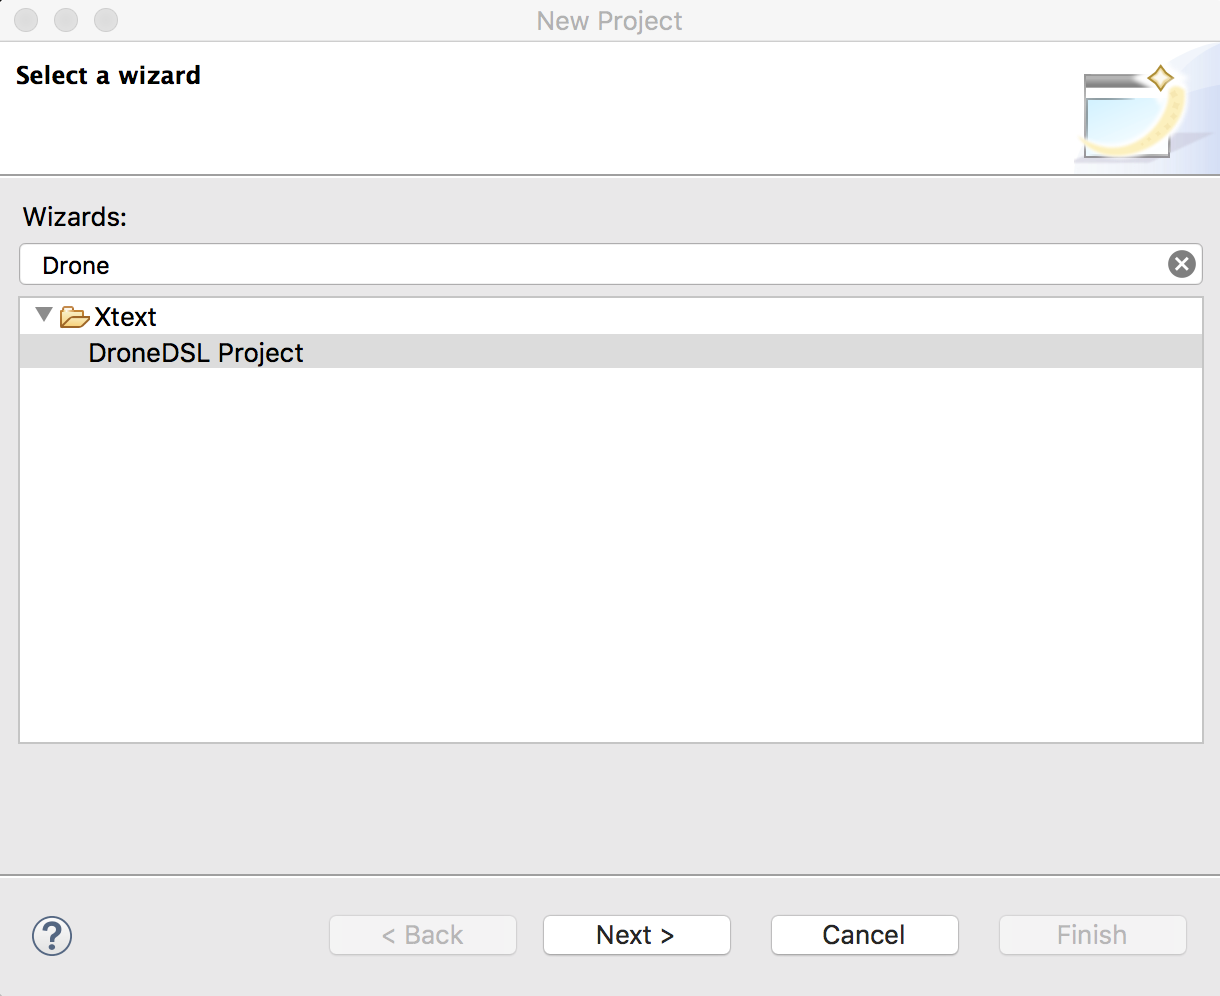
\includegraphics[scale=0.3]{images/05.png}
\caption{Création d'un nouveau projet Xtext}
\end{figure}
\end{frame}

\begin{frame}{Environnement}
\begin{block}{Création d'un projet}
\begin{itemize}
\item Création du fichier ".main\_drone" automatique.
\end{itemize}
\end{block}\pause
\begin{figure}
\centering
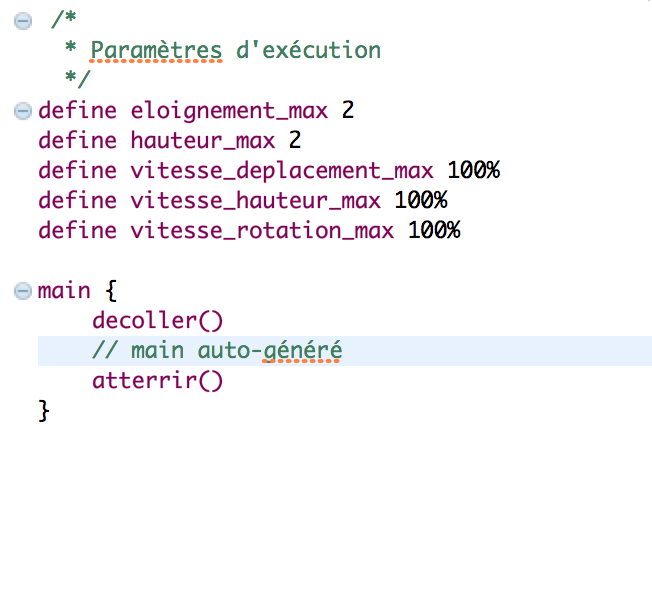
\includegraphics[scale=0.5]{images/07.png}
\caption{Fichiers auto-générés}
\end{figure}
\end{frame}

\begin{frame}{Environnement}
\begin{block}{Lancer le projet}
\begin{itemize}
\item Cliquer sur le bouton "génération" pour chaque fichier que l'utilisateur à modifier. Il peut ensuite faire un sélectionner le dossier "src" puis cliquer sur le bouton Run (Bouton play avec un fond vert) une fois qu'il n'y a plus d'erreur syntaxique.
\end{itemize}
\end{block}\pause



\begin{figure}%
    \centering
    \subfloat[Bouton génération]{{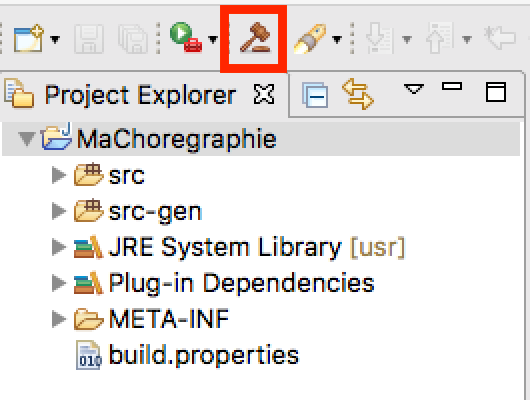
\includegraphics[width=5cm]{images/09} }}%
    \qquad
    \subfloat[Lancement]{{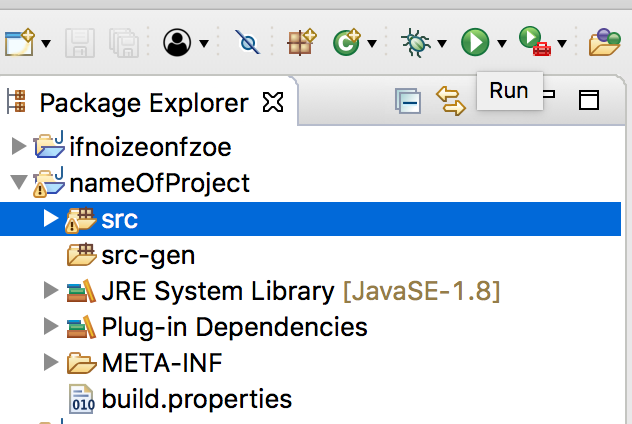
\includegraphics[width=5cm]{images/09bis} }}%
    \label{fig:example}%
\end{figure}








\end{frame}

\section{Solution}
\subsection{Solution}
\begin{frame}{Fonctionnement}
\begin{block}{Général}
	\begin{itemize}
    \item Chorégraphie écrite par l'utilisateur. \pause
    \item Chorégraphie interprétée pour générer des classes JAVA (dont la principale nommée Main). \pause
    \item La classe Main instancie les mouvements de l'utilisateur et les différents appels de fonctions. \pause
    \item La classe Runtime (JAVA) se charge de l'ouverture d'un flux de communication en direction de notre programme runtime C (déjà compilé). \pause
    \item Chaque mouvements de notre programme est envoyé au drone via notre Runtime (JAVA vers C). \pause
    \item Notre runtime C interprète ces informations et envoi des commandes au drone via l'API du constructeur.
	\end{itemize}
\end{block}
\end{frame}

\begin{frame}{Fonctionnement}
\begin{exampleblock}{Détails}
\begin{itemize}
\item Mode de fonctionnement Client/Serveur.
\item Une commande est associée à un Thread.
\item Pour les commandes parallèles, une liste de thread est associée à ces dernières.
\item Un Thread attend le temps renseigné par l'utilisateur dans sa chorégraphie avant de demander à la runtime C de d'arrêter le mouvement.
\end{itemize}
\end{exampleblock}
\end{frame}

\begin{frame}{Fonctionnement : quelques images}
\begin{figure}
\centering
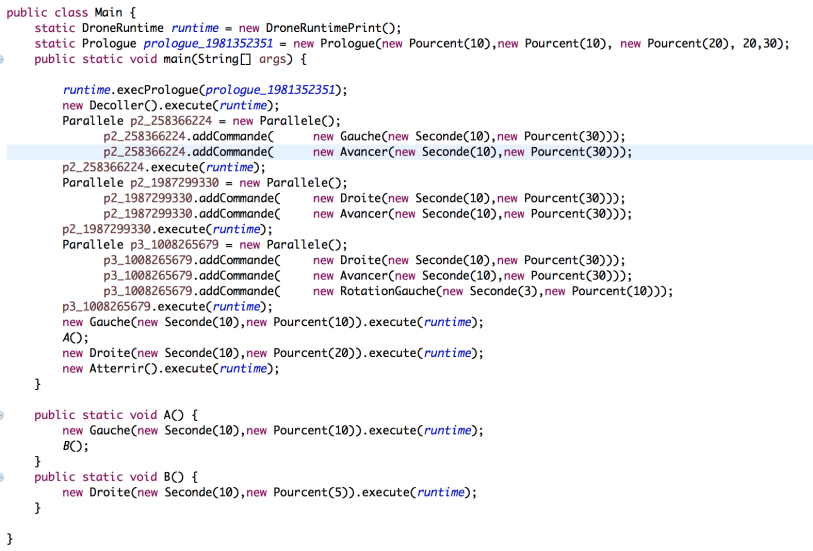
\includegraphics[scale=0.35]{images/ClasseGen.png}
\caption{Classe Main générée}
\end{figure}
\end{frame}

\begin{frame}{Fonctionnement : quelques images}
\begin{figure}
\centering
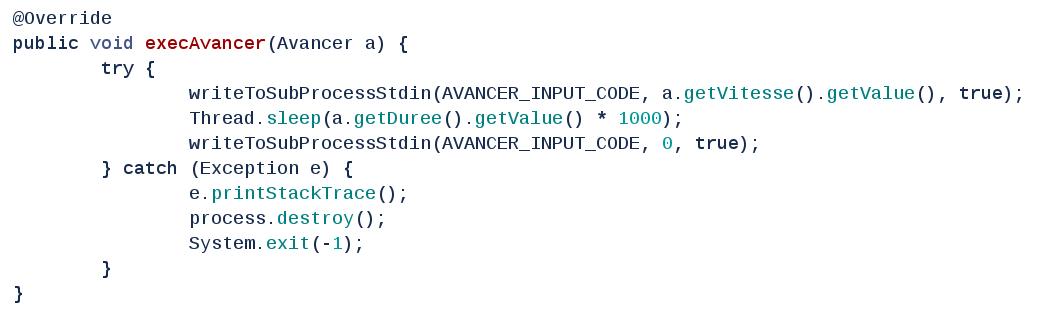
\includegraphics[scale=0.30]{images/RuntimeAvancer.png}
\caption{Exemple de la fonction Avancer de la Runtime Parrot}
\end{figure}
\end{frame}

\begin{frame}{Fonctionnement : quelques images}
\begin{figure}
\centering
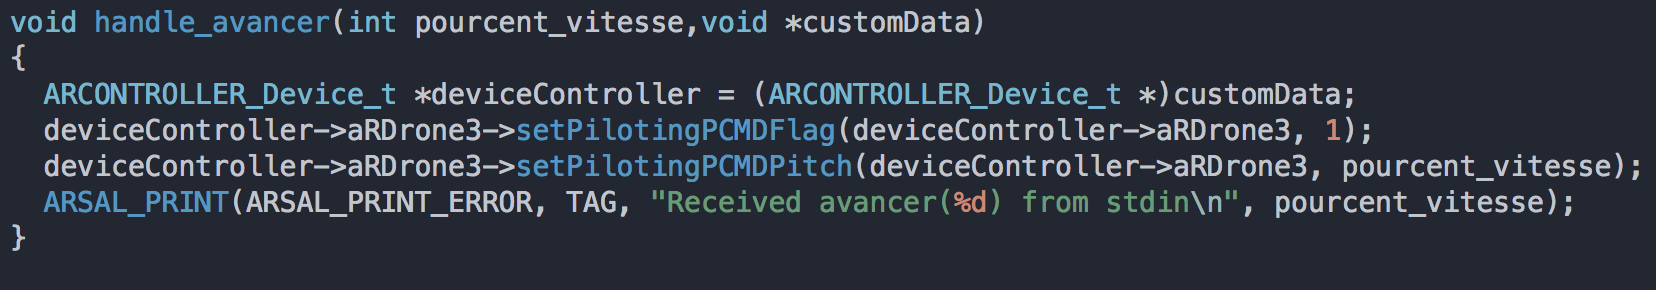
\includegraphics[scale=0.18]{images/Cavancer.png}
\caption{Exemple de la fonction Avancer de notre programme C pour Parrot}
\end{figure}
\end{frame}

\begin{frame}{Demonstration}
\centering
Démonstration
\end{frame}




\end{document}




